
% stack-permutation.tex

%%%%%%%%%%%%%%%
\begin{frame}{}
  \begin{center}
    {\LARGE Stackable Permutations}
  \end{center}
\end{frame}
%%%%%%%%%%%%%%%

%%%%%%%%%%%%%%%
\begin{frame}{}
  \begin{definition}[Stackable Permutations]
    \uncover<2->{
      \[
	\fbox{$\texttt{out} = (a_1, \cdots, a_n) \blue{\xleftarrow[\;X \;=\; \bot\;]{\;S \;=\; \emptyset\;}} \texttt{in} = (1, \cdots, n)$}
      \]
    }

    \fig{width = 0.65\textwidth}{figs/stack-perm-x}
  \end{definition}
\end{frame}
%%%%%%%%%%%%%%%

%%%%%%%%%%%%%%%
\begin{frame}{}
  \fig{width = 0.50\textwidth}{figs/stack-perm-x}

  \begin{center}
    \red{We can assume that $X$ is always blank.}
  \end{center}

  \pause
  \[
    \cyan{\texttt{read}} + \purple{\texttt{push}} \qquad
    \cyan{\texttt{read}} + \cyan{\texttt{print}}
  \]
  \[
    \purple{\texttt{pop}} + \cyan{\texttt{print}} \qquad
    \purple{\texttt{pop}} + \purple{\texttt{push}}
  \]
\end{frame}
%%%%%%%%%%%%%%%

%%%%%%%%%%%%%%%
\begin{frame}{}
  \begin{columns}
    \column{0.50\textwidth}
      \fig{width = 0.90\textwidth}{figs/stack-perm-x}
    \pause
    \column{0.50\textwidth}
      \fig{width = 0.80\textwidth}{figs/stack-perm-inout}
  \end{columns}

  \pause
  \vspace{0.40cm}
  \fig{width = 0.40\textwidth}{figs/stack-perm}
\end{frame}
%%%%%%%%%%%%%%%

%%%%%%%%%%%%%%%
\begin{frame}{}
  \begin{definition}[Stackable Permutations]
    \[
      \fbox{$\texttt{out} = (a_1, \cdots, a_n) \blue{\xleftarrow{\;S \;=\; \emptyset\;}} \texttt{in} = (1, \cdots, n)$}
    \]

    \fig{width = 0.50\textwidth}{figs/stack-perm}
  \end{definition}
\end{frame}
%%%%%%%%%%%%%%%

%%%%%%%%%%%%%%%
\begin{frame}{}
  \begin{exampleblock}{DH 2.12: Stackable Permutations}
    \begin{enumerate}[(a)]
      \item Show that the following permutations \emph{\blue{are}} stackable:
	\begin{enumerate}[(i)]
	  \item $(3, 2, 1)$
	  \item \textcolor{purple}{$(3, 4, 2, 1)$}
	  \item $(3, 5, 7, 6, 8, 4, 9, 2, 10, 1)$
	\end{enumerate}
    \end{enumerate}
  \end{exampleblock}

  \pause
  \vspace{0.50cm}
  \begin{columns}
    \column{0.50\textwidth}
      \fig{width = 0.80\textwidth}{figs/stack-perm}
    \column{0.50\textwidth}
      \fig{width = 0.80\textwidth}{figs/no-choice}
  \end{columns}
\end{frame}
%%%%%%%%%%%%%%%

%%%%%%%%%%%%%%%
\begin{frame}{}
  \begin{exampleblock}{DH 2.13: Stackable Permutations Checking Algorithm}
    To check whether a given permutation can be obtained by a stack.
  \end{exampleblock}

  \vspace{0.50cm}
  \begin{columns}
    \column{0.50\textwidth}
      \fig{width = 0.75\textwidth}{figs/stack-perm}
    \column{0.50\textwidth}
      % stack-perm-alg-no-fail.tex

\begin{algorithm}[H]
  \begin{algorithmic}[1]
    \Procedure{Stackable}{$out$}
      \ForAll{$a_j \in out$}
	\While{$\blue{\textsf{top}(S) \neq a_j}$}
	  \State \purple{$\textsf{Push}(in, S)$}
	\EndWhile
	\State \purple{$\textsf{Pop}(out, S)$}
      \EndFor
    \EndProcedure
  \end{algorithmic}
\end{algorithm}

  \end{columns}

  \pause
  \vspace{0.60cm}
  \begin{center}
    \red{\it $Q:$ What is wrong with \textsc{Stackable}?}
  \end{center}
\end{frame}
%%%%%%%%%%%%%%%

%%%%%%%%%%%%%%%
\begin{frame}{}
  \begin{exampleblock}{DH 2.13: Stackable Permutations Checking Algorithm}
    To check whether a given permutation can be obtained by a stack.
  \end{exampleblock}

  \vspace{0.50cm}
  \begin{columns}
    \column{0.40\textwidth}
      \fig{width = 0.85\textwidth}{figs/stack-perm}
    \column{0.60\textwidth}
      % stack-perm-alg-fail.tex

\begin{algorithm}[H]
  \begin{algorithmic}[1]
    \Procedure{Stackable}{$out$}
      \ForAll{$a_j \in out$}
	\While{$\blue{\textsf{top}(S) \neq a_j \land in \neq \emptyset}$}
	  \State \purple{$\textsf{Push}(in, S)$}
	\EndWhile

	\hStatex
	\If{\teal{$\textsf{top}(S) = a_j$}}
	  \State \purple{$\textsf{Pop}(out, S)$}
	\Else  \Comment{\cyan{$\textsf{top}(S) \neq a_j \land in = \emptyset$}}
	  \State \Return $F$
	\EndIf
      \EndFor

      \hStatex
      \State \Return $T$
    \EndProcedure
  \end{algorithmic}
\end{algorithm}

  \end{columns}
\end{frame}
%%%%%%%%%%%%%%%

%%%%%%%%%%%%%%%
\begin{frame}{}
  \begin{exampleblock}{DH 2.12: Stackable Permutations}
    \begin{enumerate}[(a)]
      \setcounter{enumi}{1}
    \item \red{\bf Prove} that the following permutations are \emph{\blue{not}} stackable:
	\begin{enumerate}[(i)]
	  \item $(3, 1, 2)$
	  \item $(4, 5, 3, 7, 2, 1, 6)$
	\end{enumerate}
    \end{enumerate}
  \end{exampleblock}

  \uncover<2->{
    \[
      (\red{3}, \red{1}, \red{2})
    \]

    \[
      (4, 5, 3, \red{7}, \red{2}, 1, \red{6})
    \]
  }

  \uncover<3->{
    \[
      \blue{\fbox{$\texttt{out} = \cdots a_i \cdots a_j \cdots a_k: i < j < k \land a_j < a_k < a_i$}}
    \]
  }

  \uncover<4->{
    \[
      312\text{-Pattern}
    \]
  }
\end{frame}
%%%%%%%%%%%%%%%

%%%%%%%%%%%%%%%
\begin{frame}{}
  \begin{theorem}[Stackable Permutations]
    A permutation $(a_1, \cdots, a_n)$ is stackable $\iff$ it is not the case that
    \[
      312\text{\it -Pattern}: \fbox{$\texttt{\it out} = \cdots a_i \cdots a_j \cdots a_k: i < j < k \land a_j < a_k < a_i$}
    \]
  \end{theorem}

  \vspace{0.30cm}
  \pause
  \begin{proof}
    \begin{columns}
      \column{0.45\textwidth}
        \[
	  \blue{\text{stackable} \Longrightarrow \nexists \;312\text{-Pattern}}
        \]
	\uncover<3->{
	  \[
	    \red{312\text{-Pattern} \Longrightarrow \text{non-stackable}}
	  \]
	}
      \column{0.45\textwidth}
        \[
          \blue{\nexists \;312\text{-Pattern} \Longrightarrow \text{stackable}}
        \]
	\uncover<4->{
	  \[
	    \red{\exists \;\text{algorithm}}
	  \]
	}
    \end{columns}
  \end{proof}
\end{frame}
%%%%%%%%%%%%%%%

%%%%%%%%%%%%%%%
\begin{frame}{}
  \begin{theorem}[Stackable Permutations]
    A permutation $(a_1, \cdots, a_n)$ is stackable $\iff$ it is not the case that
    \[
      312\text{\it -Pattern}: \fbox{$\texttt{\it out} = \cdots a_i \cdots a_j \cdots a_k: i < j < k \land a_j < a_k < a_i$}
    \]
  \end{theorem}

  \vspace{0.30cm}
  \begin{proof}[$312\text{-Pattern} \Longrightarrow \text{non-stackable}$]
    \begin{columns}
      \column{0.17\textwidth}
      \column{0.65\textwidth}
        \pause
	\begin{description}[$j < k \land a_j < a_k$:]
	  \item[$i < j \land a_j < a_i$:] $\textsf{Push}_{j} \quad \textsf{Push}_{i} \quad \textsf{Pop}_{i} \quad \textsf{Pop}_{j}$
	  \item[$j < k \land a_j < a_k$:] $\textsf{Push}_{j} \quad \textsf{Pop}_{j} \quad \textsf{Push}_{k} \quad \textsf{Pop}_{k}$
	  \item[$i < k \land a_k < a_i$:] $\textsf{Push}_{k} \quad \textsf{Push}_{i} \quad \textsf{Pop}_{i} \quad \textsf{Pop}_{k}$
	\end{description}
      \column{0.17\textwidth}
    \end{columns}
  \end{proof}
\end{frame}
%%%%%%%%%%%%%%%

%%%%%%%%%%%%%%%
\begin{frame}[fragile]{}
  \begin{theorem}[Stackable Permutations]
    A permutation $(a_1, \cdots, a_n)$ is stackable $\iff$ it is not the case that
    \[
      312\text{\it -Pattern}: \fbox{$\texttt{\it out} = \cdots a_i \cdots a_j \cdots a_k: i < j < k \land a_j < a_k < a_i$}
    \]
  \end{theorem}

  \begin{proof}[$\nexists \;312\text{-Pattern} \Longrightarrow \text{Obtainable by \textsc{Stackable}}$]

    \uncover<2->{
      \begin{center}
	\red{\textsc{Stackable} fails $\implies \exists \;312\text{-Pattern}$.}
      \end{center}
    }

    \vspace{-0.50cm}
    \begin{columns}
      \column{0.60\textwidth}
        % stack-perm-alg-fail.tex

\begin{algorithm}[H]
  \begin{algorithmic}[1]
    \Procedure{Stackable}{$out$}
      \ForAll{$a_j \in out$}
	\While{$\blue{\textsf{top}(S) \neq a_j \land in \neq \emptyset}$}
	  \State \purple{$\textsf{Push}(in, S)$}
	\EndWhile

	\hStatex
	\If{\teal{$\textsf{top}(S) = a_j$}}
	  \State \purple{$\textsf{Pop}(out, S)$}
	\Else  \Comment{\cyan{$\textsf{top}(S) \neq a_j \land in = \emptyset$}}
	  \State \Return $F$
	\EndIf
      \EndFor

      \hStatex
      \State \Return $T$
    \EndProcedure
  \end{algorithmic}
\end{algorithm}

      \column{0.50\textwidth}
      \uncover<3->{
	\[
	  a_j \neq \textsf{top}(S) \land in = \emptyset 
	\]
      }
      \vspace{-0.30cm}
      \uncover<4->{
	\[
	  \red{\it a_j \text{ is covered by some } a_k \text{ in } S}
	\]
      }
      \vspace{-0.30cm}
      \uncover<5->{
	\[
	 \exists k: j < k \land a_j < a_k
	\]
      }
      \vspace{-0.30cm}
      \uncover<6->{
	\[
	  \red{\it \text{Why is } a_k \text{ in } S?}
	\]
      }
      \vspace{-0.30cm}
      \uncover<7->{
	\[
	 \exists i: i < j \land a_k < a_i
	\]
      }
    \end{columns}
  \end{proof}
\end{frame}
%%%%%%%%%%%%%%%

%%%%%%%%%%%%%%%
\begin{frame}{}
  \begin{exampleblock}{DH 2.12: Stackable Permutations}
    \begin{enumerate}[(a)]
      \setcounter{enumi}{2}
      \item How many permutations of $A_4$ \red{\emph{cannot}} be obtained by a stack?
    \end{enumerate}
  \end{exampleblock}

  \begin{align*}
    &(1, \redoverlay{4}{2-}, \redoverlay{2}{2-}, \redoverlay{3}{2-}), (2, 4, 1, 3), (3, 1, 2, 4), 
    (\redoverlay{3}{2-}, \redoverlay{1}{2-}, 4, \redoverlay{2}{2-}), (3, 4, 1, 2) \\
    &(4, 1, 2, 3), (4, 1, 3, 2), (\redoverlay{4}{2-}, 2, \redoverlay{1}{2-}, \redoverlay{3}{2-}), (4, 2, 3, 1), (4, 3, 1, 2)
  \end{align*}

  \vspace{0.60cm}
  \uncover<3->{
    \begin{center}
      {\red{\it $Q:$ What about $A_n$?}}
    \end{center}
  }
\end{frame}
%%%%%%%%%%%%%%%

%%%%%%%%%%%%%%%
\begin{frame}{}
  \begin{exampleblock}{DH 2.12: Stackable Permutations}
    How many permutations of $\set{1 \cdots n}$ are stackable?
  \end{exampleblock}

  \fig{width = 0.50\textwidth}{figs/stack-perm}

  \pause
  \centerline{\red{$Q:$} How many \blue{\emph{admissible}} operation sequences of \purple{``\texttt{Push}''} and \purple{``\texttt{Pop}''}?}
\end{frame}
%%%%%%%%%%%%%%%

%%%%%%%%%%%%%%%
\begin{frame}{}
  \begin{definition}[Admissible Operation Sequences]
    An operation sequence of \purple{``\texttt{Push}''} and \purple{``\texttt{Pop}''} is \blue{\it admissible} if and only if
    \begin{enumerate}[(i)]
      \pause
      \item $\# \text{ of ``\texttt{Push}''} = n \qquad \# \text{ of ``\texttt{Pop}''} = n$
      \pause
      \item $\forall \text{ prefix}: (\# \text{ of ``\texttt{Pop}''}) \le (\# \text{ of ``\texttt{Push}''})$
    \end{enumerate}
  \end{definition}

  \vspace{0.50cm}
  \pause
  \begin{center}
    \red{\fbox{\# of admissible operation sequences $=$ \# of stackable perms}}
  \end{center}

  \pause
  \[
    \set{\text{admissible operation sequences}} \xrightarrow{\exists f: 1-1} \set{\text{stackable perms}}
  \]

  \pause
  \[
    f(s) \triangleq \text{\red{\it Execute} this admissible operation sequence } s
  \]

  \pause
  \begin{center}
    \red{\it Why is $f$ bijective (1-1)?}
  \end{center}
\end{frame}
%%%%%%%%%%%%%%%

%%%%%%%%%%%%%%%
% \begin{frame}{}
%   \begin{theorem}
%     Different admissible operation sequences correspond to different permutations.
%   \end{theorem}
% 
%   \vspace{0.30cm}
%   \pause
%   \begin{proof}
%     \begin{align*}
%       &\push{}\; \;\push{}\; \;\push{}\; \;\pop{}\; \;\pop{}\; \;\red{\push{}} \cdots \\
%       &\push{}\; \;\push{}\; \;\push{}\; \;\pop{}\; \;\pop{}\; \;\red{\pop{}} \cdots \\
%     \end{align*}
%   \end{proof}
% \end{frame}
%%%%%%%%%%%%%%%

%%%%%%%%%%%%%%%
\begin{frame}{}
  \begin{theorem}
    The number of admissible operation sequences of \texttt{\it \purple{``Push''}} and \texttt{\it \purple{``Pop''}} is ${2n \choose n} - {2n \choose n-1}$.
  \end{theorem}

  \pause
  \begin{proof}[Proof: The Reflection Method]
    \[
      \push{}: \;\rightarrow \qquad \pop{}: \;\uparrow
    \]

    \begin{columns}
      \pause
      \column{0.50\textwidth}
	% \fig{width = 0.90\textwidth}{figs/grid-path}
	\begin{center}
	  \resizebox{0.80\textwidth}{!}{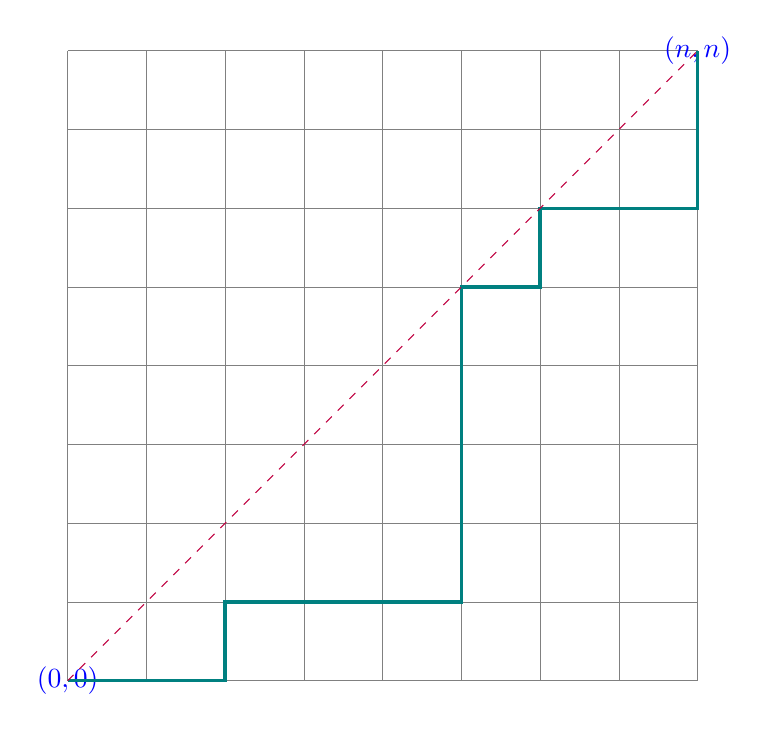
\begin{tikzpicture}
  \draw[help lines] (0,0) grid (8,8);

  \node (00) [blue] {$(0,0)$};
  \node (nn) [blue] at (8,8) {$(n,n)$};

  \pause
  \draw[teal, very thick] (0,0) -- (1,0) -- (2,0) 
    -- (2,1) -- (3,1) -- (4,1) -- (5,1) 
    -- (5,2) -- (5,3) -- (5,4) -- (5,5)
    -- (6,5) -- (6,6)
    -- (7,6) -- (8,6)
    -- (8,7) -- (8,8);

  \pause
  \draw[purple, dashed] (00.center) to (nn.center);
\end{tikzpicture}
}
	\end{center}
      \column{0.50\textwidth}
	\uncover<6->{
	  \[
	    \blue{\underbrace{\textcolor{black}{{2n \choose n}}}_{\text{all}}} 
	    - \red{\underbrace{\textcolor{black}{{2n \choose n-1}}}_{\text{inadmissible}}}
	  \]
	}
    \end{columns}
  \end{proof}
\end{frame}
%%%%%%%%%%%%%%%

%%%%%%%%%%%%%%%
\begin{frame}{}
  \begin{center}
    \resizebox{0.60\textwidth}{!}{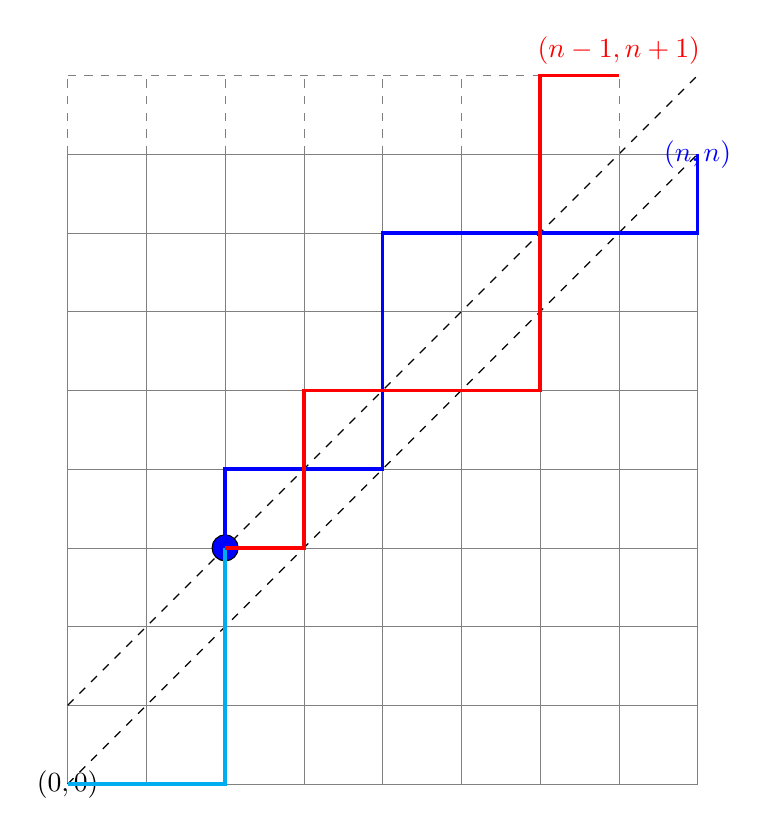
\begin{tikzpicture}
  \draw[help lines] (0,0) grid (8,8);

  \node (00) [] {$(0,0)$};
  \node (01) [] at (0,1) {};
  \node (nn) [blue] at (8,8) {$(n,n)$};

  \draw [dashed] (0,0) to (8,8);

  \pause
  \draw[very thick] (0,0) -- (1,0) -- (2,0) --
	(2,1) -- (2,2) -- (2,3);
  \draw[very thick] (2,3) -- (2,4) --
	(3,4) -- (4,4) --
	(4,5) -- (4,6) -- (4,7) --
	(5,7) -- (6,7) -- (7,7) -- (8,7) --
	(8,8);

  \pause
  \node (nn1) [] at (8,9) {};
  \draw [dashed] (0,1) to (8,9);

  \pause
  \node () [circle, draw, fill = blue] at (2,3) {};

  \pause
  \draw[very thick, cyan] (0,0) -- (1,0) -- (2,0) --
	(2,1) -- (2,2) -- (2,3);
  \draw[very thick, blue] (2,3) -- (2,4) --
	(3,4) -- (4,4) --
	(4,5) -- (4,6) -- (4,7) --
	(5,7) -- (6,7) -- (7,7) -- (8,7) --
	(8,8);

  \pause
  \draw[help lines, dashed] (0,8) grid (7,9);
  \draw[very thick, red] 
	(2,3) -- (3,3) --
	(3,4) -- (3,5) --
	(4,5) -- (5,5) -- (6,5) --
	(6,6) -- (6,7) -- (6,8) -- (6,9) --
	(7,9) node[above] () {$(n-1, n+1)$};
\end{tikzpicture}}
  \end{center}
\end{frame}
%%%%%%%%%%%%%%%

%%%%%%%%%%%%%%%
% \begin{frame}{}
%   \begin{center}
%     \resizebox{0.60\textwidth}{!}{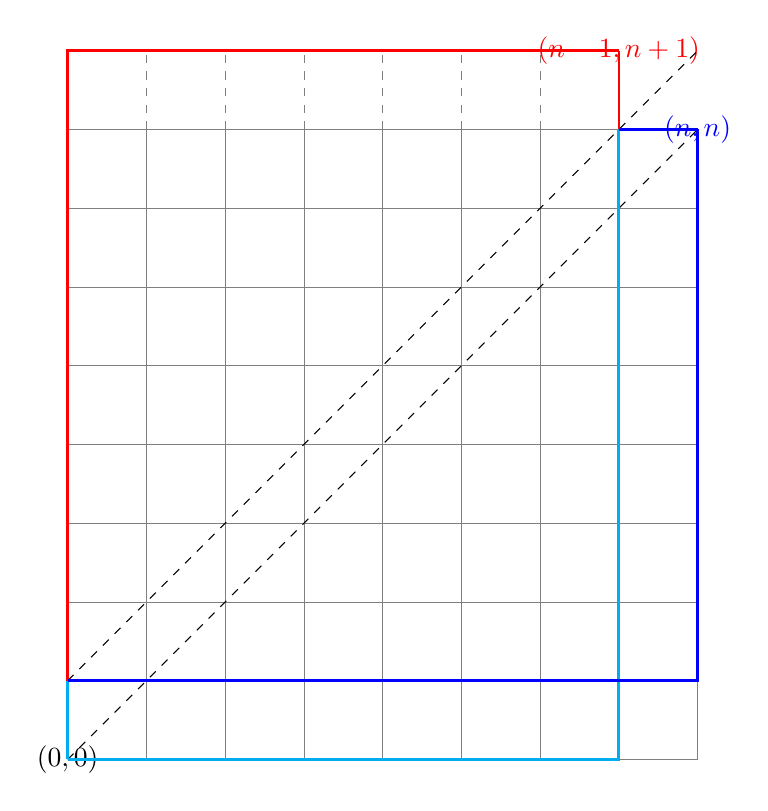
\begin{tikzpicture}
  \draw[help lines] (0,0) grid (8,8);
  \draw[help lines, dashed] (0,8) grid (7,9);

  \node (00) [] {$(0,0)$};
  \node (01) [] at (0,1) {};
  \node (nn) [blue] at (8,8) {$(n,n)$};
  \node (nn1) [] at (8,9) {};
  \node (n1n1) [red] at (7,9) {$(n-1, n+1)$};

  \draw [dashed] (0,0) to (8,8);
  \draw [dashed] (0,1) to (8,9);

  \uncover<2-3>{
    \draw[very thick, cyan] (0,0) -- (7,0) -- (7,8);
  \draw[thick, red] (7,8) -- (7,9);
  }
  \uncover<3>{
    \draw[very thick, blue] (7,8) -- (8,8);
  }

  \uncover<4-5>{
    \draw[very thick, cyan] (0,0) -- (0,1);
    \draw[very thick, red] (0,1) -- (0,9) -- (7,9);
  }
  \uncover<5>{
    \draw[very thick, blue] (0,1) -- (8,1) -- (8,8);
  }
\end{tikzpicture}
}
%   \end{center}
% \end{frame}
%%%%%%%%%%%%%%%

%%%%%%%%%%%%%%%
\begin{frame}{}
  \[
    {2n \choose n} - {2n \choose n-1}
  \]

  \begin{center}
    {\Large \href{https://en.wikipedia.org/wiki/Catalan\_number}{Catalan Number}}
  \end{center}

  \[
    (3,2,1): ((())) \qquad (1,2,3): ()()()
  \]
\end{frame}
%%%%%%%%%%%%%%%